\chapter{Test dei metodi di spam detection}
\lstset{basicstyle=\small\ttfamily,keywordstyle=\color{black}\bfseries,commentstyle=\color{darkgray},stringstyle=\color{black},showstringspaces=true} 
Nei capitoli precedenti sono stati illustrati vari metodi di spam detection classificati in base a segnali in ingresso utilizzati; quindi sono state identificate tre classi: metodi basati sul contenuto, metodi basati sul grafo e metodi che utilizzano segnali diversi dai primi due. Nell'analisi che è stata eseguita sono sono stati presi in esame due algoritmi di spam detection basati sul grafo che operano offline: \textit{Trustrank} e \textit{Anti-trust rank}. 

Si è scelto, quindi, di valutare l'efficacia di due  algoritmi \textit{link based} offline (\textit{Trustrank} e \textit{Anti-trust rank}) durante l'operazione di crawling ovvero in modo online. In particolare i vari test consistono nel verificare quanto questi due algoritmi di tipo offline riescano ad approssimare il loro comportamento se li facessimo operare in modo online (quindi durante la fase di crawling). Le domande che ci poniamo eseguendo questi test su i due algoritmi di spam detection offline (\textit{Trustrank} e \textit{Anti-trus rank}) sono:
\begin{itemize}
 \item possono questi algoritmi essere in grado di operare in modalità online?
 \item durante l'esecuzione in modalità online, quanto riescono ad approssimare il loro comportamento offline?
 \item è conveniente utilizzare questi algoritmi in modalità online?
\end{itemize}

E' doveroso specificare che un algoritmo di spam detection lavora offline se questo viene eseguito dopo l'attività di crawling (e quindi dopo che si ha a disposizione l'intero grafo ottenuto dai collegamenti tra le pagine), mentre un algoritmo di spam detection lavora online se questo viene eseguito durante il processo di crawling e quindi riesce a determinare all'istante se una pagina deve essere considerata spam o non spam. Dal momento che si è scelto di esaminare degli algoritmi \textit{linked base}, e sapendo che questi formulano delle conclusioni sulla natura delle pagine (ovvero se sono spam o non spam) esaminando la struttura dell'intero grafo, è interessante notare come questi algoritmi si comportino se il grafo su cui vengono fatte le valutazioni è incompleto.
%altre considerazioni

Il capitolo, quindi, è diviso nel seguente modo: nella prima parte verrà illustrata la tecnica di simulazione il crawler in modo tale da eseguire gli algoritmi offline durante la fase di crawling; nella seconda parte verrà spiegato come sono stati implementati i test; nell'ultima parte verrano illustrati tutti i risultati ottenuti.

\section{Simulazione del crawler}
Per simulare il comportamento di un crawler, e quindi eseguire gli algoritmi di \textit{Trustrank} e \textit{Anti-trust rank} in modalità online, abbiamo implementato una semplice visita in ampiezza sul grafo ovvero una BFS \cite{bfsCormen} (Breadth-First Search). La visita in ampiezza dato un grafo \(G=(V,E)\), dove \(V\) è l'insieme dei vertici del grafo ed \(E\) l'insieme degli archi del grafo, e un vertice \(s\) da cui far partire la visita, scopre tutti i vertici che sono raggiungibili da \(s\). La visita in ampiezza scopre tutti i vertici che si trovano a distanza \(f\) dal vertice di partenza e successivamente scopre i vertici che si trovano a una distanza successiva \(f+1\). In sostanza dato il nodo di partenza \(s\), la visita in ampiezza, scopre tutti i nodi vicini al nodo \(s\) e successivamente per ogni nodo vicino scoperto trova i vicini che non sono ancora stati visitati; questo processo viene iterato finché tutti i nodi del grafo raggiungibili da \(s\) sono visitati. \\
Il framework WebGraph mette a disposizione un'implementazione efficiente della visita in ampiezza, in particolare  la classe ``ParallelBreadthFirstVisit'' esegue una visita in ampiezza utilizzando il parallelismo derivato dai processori multicore.

\section{I test}
Come anticipato lo scopo dei test è analizzare il comportamento degli algoritmi \textit{trustrank} e \textit{anti-trust rank} durante la fase di crawling ovvero in modalità online. Gli algoritmi \textit{linked base} quali \textit{trustrank} e \textit{anti-trust rank} in modalità online operano su un grafo del web incompleto all'inizio del crawling, fino ad arrivare ad operare sull'intero grafo alla fine del crawling.

\begin{figure}
\centering
 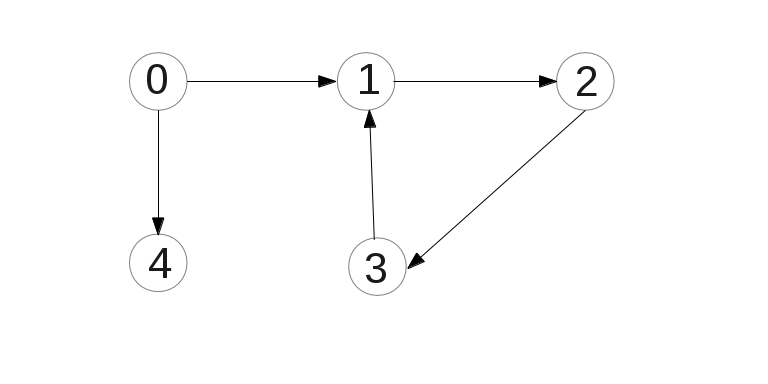
\includegraphics{immagini/test/grafoComp}
 \caption{Esempio di grafo}
 \label{fig:grafoComp}
\end{figure}

Quasi tutti i test seguono uno stesso schema; viene calcolato il vettore \(t\) di  \textit{Trustrank} (e il vettore \(a\) di \textit{Anti-trust rank}) sull'intero grafo \(G\) che è il grafo degli host ricavato dal dataset; successivamente viene eseguita la visita in ampiezza \(v\) con nodo sorgente \(s\) e quindi si ricava la coda \(q\) dei nodi visitati a partire da \(s\); dopo di che si calcola  \textit{Trustrank} (e \textit{Anti-trust rank}) sul grafo temporaneo \(G_v\), questo grafo è ottenuto lungo la visita in ampiezza \(v\) ed è formato, quindi, da un sottoinsieme di nodi \(q\); il vettore di \textit{trustrank} calcolato sul grafo temporaneo lo indicheremo con \(\hat{t}_i\) (mentre il vettore di \textit{anti-trust rank} sarà indicato con \(\hat{a}_i\)) dove \(i\) è il numero di nodi visitati ad un certo passo della visita. Questo processo viene iterato incrementando sempre di più l'intervallo \(i\) finché non si arriva alla fine della coda \(q\) dei nodi visitati partendo dal nodo \(s\). Infine viene 
calcolata la distanza tra i due vettori \(t\) e \(\hat{t}_i\) tramite la Tau di Kendall e indicheremo con \(\tau_t(t,\hat{t}_i)\) la Tau di Kendall per \(t\) e \(\hat{t}_i\)  (e quindi \(\tau_a(a,\hat{a}_i)\) sarà la Tau di Kendall per \(a\) e \(\hat{a}_i\)). Ad esempio in figura \ref{fig:grafoComp} è rappresentato il grafo completo su cui verrà calcolato \(t\) e \(a\) mentre in figura \ref{fig:grafo3} è rappresentato il grafo temporaneo ricavato dalla visita in ampiezza eseguita sul grafo precedente partendo dal nodo 1. Se si considerano tutti i nodi incontrati lungo la visita il vettore di \textit{trustrank} calcolato sul grafo temporaneo alla fine della visita sarà \(\hat{t}_3\) mentre quello di \textit{anti-trust rank} sarà \(\hat{a}_3\).

 \begin{figure}
\centering
 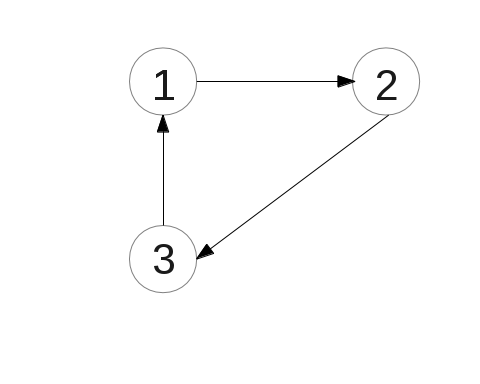
\includegraphics{immagini/test/grafo3}
 \caption{Esempio di grafo ricavato tramite una BFS a partire dal nodo 1 del grafo in figura \ref{fig:grafoComp}.}
 \label{fig:grafo3}
\end{figure}
A ogni indice del  vettore di \textit{Trustrank} \(t\), calcolato sull'intero grafo \(G\), e del vettore di \textit{Anti-trust rank} \(a\), calcolato sull'intero grafo \(G\), corrisponderà un nodo e il valore assegnato ad ogni  indice indica il valore di \textit{Trustrank} e \textit{Anti-trust rank} del nodo del grafo \(G\). In figura \ref{fig:tVettore} è illustrato un esempio del vettore di \textit{trustrank} calcolato sull'intero grafo e in figura \ref{fig:aVettore} è illustrato un esempio del vettore di \textit{anti-trust rank} calcolato sull'intero grafo. 
Nell'esempio in figura \ref{fig:tVettore} si nota che il vettore \(t\) di \textit{trustrank} ha lunghezza 5, quindi il grafo sarà composto da 5 nodi dove ad ogni nodo è associato il valore di \textit{trustrank}. Le stesse considerazioni valgono per l'esempio in figura \ref{fig:aVettore} dove il vettore di \textit{anti-trust rank} è ha lunghezza 5 e quindi l'algoritmo opererà su un grafo composto da 5 nodi.

\begin{figure}
\centering
 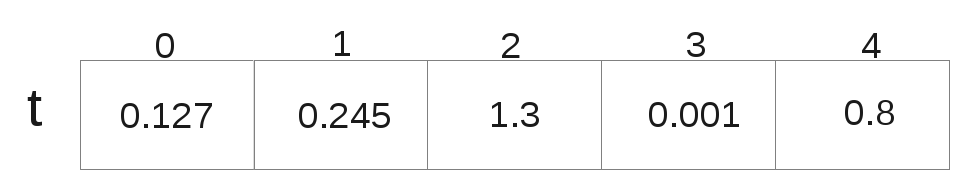
\includegraphics{immagini/test/trustVettore}
 \caption{Esempio del vettore di trustrank calcolato sull'intero grafo}
 \label{fig:tVettore}
\end{figure}
\begin{figure}
\centering
 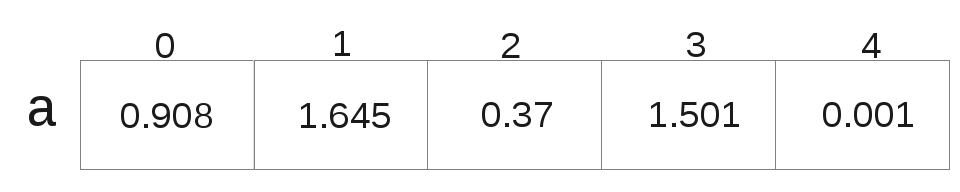
\includegraphics{immagini/test/immagineAntiTrust}
 \caption{Esempio del vettore di anti-trust rank calcolato sull'intero grafo}
 \label{fig:aVettore}
\end{figure}

A differenza dei vettori \(t\) e \(a\) calcolati sull'intero grafo \(G\) dove ad ogni indice è associato un valore di \textit{trustrank} e \textit{anti-trust rank} , i vettori \(\hat{t}_i\) e \(\hat{a}_i\) calcolati sul grafo temporaneo \(G_v\) di solito non hanno la stessa lunghezza. Più precisamente, sapendo che \(\hat{t}_i\) e \(\hat{a}_i\) sono calcolati sul grafo temporaneo \(G_v\) durante l'esecuzione di una visita in ampiezza \(v\), allora se \(v\) non ha terminato la visita ci saranno ancora dei nodi da visitare per cui non è possibile calcolare i valori di \textit{trustrank} e \textit{anti-trust rank}. Quindi con l'avanzamento della visita in ampiezza sempre più nodi avranno associato un valore di \textit{trustrank} e \textit{anti-trust rank}; cioè \(\hat{t}_i\) e \(\hat{a}_i\), con l'avanzamento della visita, avranno una lunghezza sempre più prossima a quella dei vettori \(t\) e \(a\). Vale quindi che \(\hat{t}_{i+1}\) avrà molti più nodi per cui è stato calcolato \textit{trustrank} rispetto a \(\
hat{t}_i\) (lo stesso comportamento si riscontra per \textit{anti-trust rank}). Inoltre non è detto che dopo aver terminato la visita in ampiezza, partendo da un nodo \(s\), si sia visitato tutto il grafo (ovvero che \(s\) può raggiungere tutti i nodi del grafo) perciò in questo caso al termine della visita i vettori \(\hat{t}_i\) e \(\hat{a}_i\) avranno un numero minore di nodi per cui è stato calcolato \textit{trustrank} e \textit{anti-trust rank} rispetto a \(t\) e \(a\).\\
Dal momento che la Tau di Kendall tra due vettori, per essere eseguita, richiede che i due vettori abbiano la stessa lunghezza allora bisogna gestire i casi in cui il numero di nodi del grafo temporaneo \(G_v\) sia più piccolo rispetto al numero di nodi dell'intero grafo \(G\).  Per gestire tale problema si è scelto di considerare i soli nodi compresi nel grafo temporaneo. Ad esempio in figura \ref{fig:tBFSmodoB} viene illustrato il caso in cui eseguendo la visita in ampiezza dal nodo 1, i nodi 0 e 4 rimangano senza aver assegnato un valore di \textit{trustrank}. Quindi gli indici 0 e 4 del vettore \(t\) non sono inclusi nel vettore \(\hat{t}_3\) questo implica che ci deve essere una corrispondenza tra gli indici del vettore \(t\) e quelli del vettore \(\hat{t}_3\) (in figura \ref{fig:tBFSmodoB} l'indice 0 del vettore \(\hat{t}_3\) corrisponde all'indice 1 del vettore \(t\), l'indice 1 al indice 2 ed infine l'indice 2 all'indice 3).  Inoltre  il vettore \(\hat{t}_3\) ha lunghezza inferiore al vettore \(t\). 
Quando il vettore \(t\) ha lunghezza maggiore del vettore \(\hat{t}_i\) il calcolo della Tau di Kendall tra il vettore \(t\) e il vettore \(\hat{t}_i\) avverrà tra i soli indici del vettore \(t\) compresi nel vettore \(\hat{t}_i\). Quindi  nella valutazione  il vettore \(t\) dovrà essere ristretto alla lunghezza del vettore \(\hat{t}_i\) e quindi dovranno essere eliminati gli indici del vettore \(t\) che non sono inclusi nel vettore \(\hat{t}_i\).
\begin{figure}
\centering
 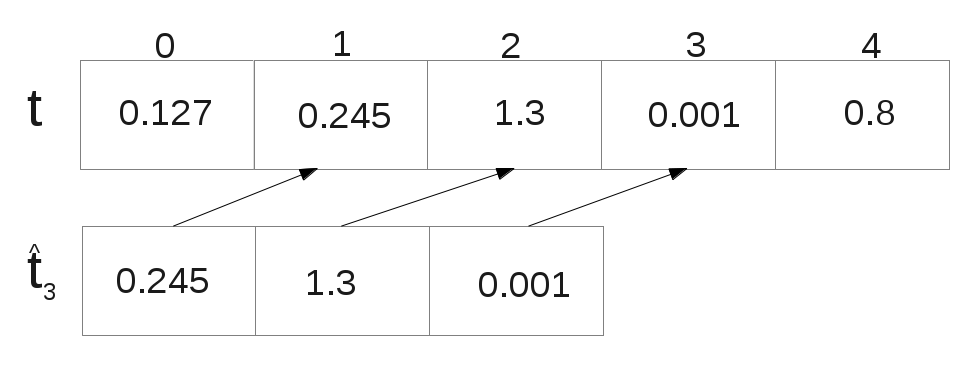
\includegraphics{immagini/test/tBFSmodoB}
 \caption{Esempio del vettore di trustrank calcolato su una porzione di grafo.}
 \label{fig:tBFSmodoB}
\end{figure}

Oltre la metodo descritto per gestire i nodi non ancora visitati può essere utilizzato un altro che consiste nell'assegnare ad ogni indice dei vettori \(\hat{t}_i\) e \(\hat{a}_i\) non ancora visitati il valore 0.0. Ad esempio prendendo in considerazione il grafo in figura \ref{fig:grafoComp} e ipotizzando di eseguire una visita in ampiezza a partire dal nodo 1 e di aver visitato i nodi 2 e 3  se calcoliamo \textit{trustrank} e \textit{anti-trust rank} sul sottografo ricavato dai nodi visitati, i nodi 0 e 4 avranno associato i valori 0.0, tale esempio è illustrato in figura \ref{fig:tBFSmodoA} e in figura \ref{fig:aBFSmodoA}. Questa metodo però è poco significativo in quanto vengono introdotti dei valori non veritieri che producono rumore, e quindi non verrà preso in considerazione.
\begin{figure}
\centering
 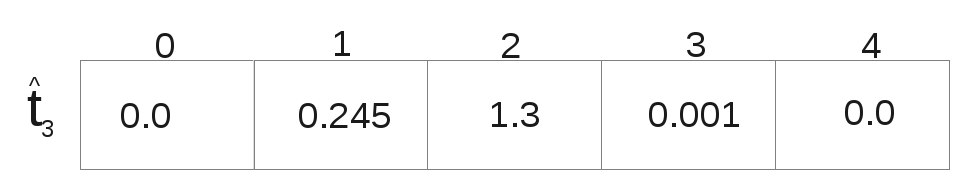
\includegraphics{immagini/test/tBFSmodoA}
 \caption{Esempio del vettore di trustrank calcolato su una porzione di grafo a cui viene assegnato il valore 0.0 ai nodi non visitati.}
 \label{fig:tBFSmodoA}
\end{figure}
\begin{figure}
\centering
 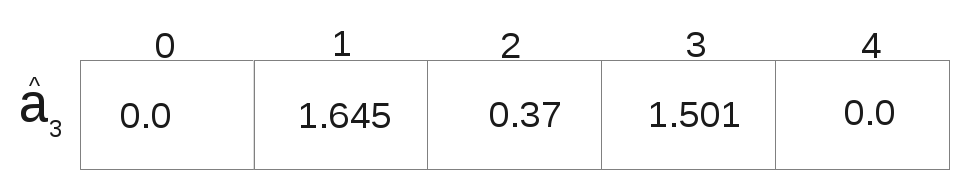
\includegraphics{immagini/test/aBFSmodoA}
 \caption{Esempio del vettore di anti-trust rank calcolato su una porzione di grafo a cui viene assegnato il valore 0.0 ai nodi non visitati.}
 \label{fig:aBFSmodoA}
\end{figure}

I test saranno, quindi, cosi strutturati:
\begin{itemize}
 \item Test numero 1. Viene calcolata la Tau di Kendall tra il  vettore \(t\) di \textit{trustrank} calcolato sul grafo completo \(G\) con il vettore \(\hat{t}_i\) di \textit{trustrank} calcolato sul grafo temporaneo \(G_v\) ricavato tramite i nodi visitati dalla visita in ampiezza. Tale processo viene ripetuto ad ogni intervallo di nodi visitato tramite la visita in ampiezza fino al termine della visita. Lo stesso processo è eseguito per valutare \textit{anti-trust rank}.
 
 \item Test numero 2. Si calcola la Tau di Kendall tra il vettore \(t\)  di \textit{trustrank} calcolato sul grafo completo \(G\) con il vettore \(\hat{t}_i\) di \textit{trustrank} calcolato sul grafo temporaneo \(G_v\) ricavato tramite i nodi visitati dalla visita in ampiezza, prendendo in considerazione i soli nodi etichettati spam.  Tale processo viene ripetuto ad ogni intervallo di nodi visitato tramite la visita in ampiezza fino al termine della visita. Nel caso di \textit{anti-trust rank} si  confrontano i nodi etichettati come non spam.
 
 \item Test numero 3. Si esegue una visita in ampiezza \(v_1\) sul grafo \(G\) con nodo sorgente \(s\). Si calcola il vettore \(t_{v1}\) di \textit{trustrank} sul grafo \(G_{v1}\) formato dai nodi visitati al termine della visita usando come seedset l'insieme \(S\) formato dagli ultimi \(n\) nodi incontrati nella visita. Successivamente si esegue una visita in ampiezza \(v_2\) sul grafo \(G\) con nodo sorgente \(s\) e si calcola il vettore di \textit{trustrank} \(\hat{t}_i\) sul grafo temporaneo \(G_{v2}\), ottenuto ad ogni intervallo di nodi incontrati dalla visita \(v_2\), usando come seedset \(S\). Dopo di che si calcola la Tau di Kendall tra \(t_{v1}\) e \(\hat{t}_i\). Tale processo viene ripetuto ad ogni intervallo di nodi visitato tramite la visita in ampiezza fino al termine della visita. Lo stesso processo è eseguito per valutare \textit{anti-trust rank}.
 
 \item Test numero 4. Viene rieseguito il \textit{test numero 3} ma con il fattore di attenuazione \(\alpha\), utilizzato nel calcolo di \textit{trustrank} e \textit{anti-trust rank} impostato a 0.0005.
 
 \item Test numero 5. Si esegue una visita in ampiezza a partire dal nodo \(s\) e ad ogni intervallo di nodi visitati si calcola la media dei valori di \textit{trustrank} dei soli nodi che sappiamo essere non spam e la media dei valori di \textit{trustrank} dei soli nodi spam. Quindi si calcola la differenza tra le due medie. Il processo verrà iterato fino alla fine della visita in ampiezza. Lo stesso metodo verrà applicato per l'analisi dell'algoritmo di \textit{anti-trust rank}.
 
 \item Test numero 6. Si riesegue il \textit{test numero 5} ma invece di usare dei valori temporanei di \textit{trustrank} e \textit{anti-trust rank} a ogni passo della visita per calcolare le relative medie, si utilizzano i valori finali del vettore \(t\) di \textit{trustrank} e del vettore  \(a\) di \textit{anti-trust rank} calcolati sull'intero grafo.
 \end{itemize}
 
\section{Test 1}
 Il test calcola la distanza, attraverso l'utilizzo  della Tau di Kendall \(\tau_t\), tra il vettore \(t\) di \textit{trustrank} ricavato sull'intero grafo \(G\) e il vettore \(\hat{t}_i\) di \textit{trustrank} calcolato sul grafo temporaneo \(G_v\) ricavato ad ogni intervallo di nodi visitati lungo una visita in ampiezza \(v\) con nodo sorgente \(s\). Il test, inoltre, valuta anche \textit{anti-trust rank}, utilizzano  la Tau di Kendall \(\tau_a\), calcola la distanza  tra il vettore \(a\) di \textit{anti-trust rank} ottenuto dal grafo completo \(G\) e il vettore \(\hat{a}_i\)  calcolato sul grafo temporaneo \(G_v\). Il calcolo delle due Tau di Kendall avviene ad ogni intervallo di nodi visitato tramite la visita in ampiezza e viene iterato finché la visita \(v\) non termina.
 I nodi sorgenti della visita in ampiezza sono due: il nodo 62 etichettato non spam e il nodo 112 etichettato spam presenti nel dataset. L'intervallo di nodi da cui si ricava il grafo temporaneo è 5000; quindi ogni 5000 nodi visitati, tramite la visita in ampiezza \(v\), si ricava il grafo temporaneo \(G_v\); perciò dopo il primo passo della visita \(v\), dove il grafo temporaneo è formato dal solo nodo sorgente, al secondo passo \(G_v\) sarà formato da 5001 nodi al terzo passo di 10001 nodi e cosi via. Inoltre durante il calcolo di \(t\) sull'intero grafo \(G\) viene utilizzato come seedset l'insieme di pagine del dataset WEBSPAM-UK2007 etichettate  non spam mentre il seedset usato nel calcolo di \(\hat{t}_i\)  sarà formato dalle pagine visitate etichetta non spam all'interno del grafo temporaneo \(G_v\). Per il calcolo del vettore \(a\) di \textit{anti-trust rank} sull'intero grafo \(G\), invece, il seedset sarà composto dalle pagine etichettate spam nel dataset WEBSPAM-UK2007 mentre il seedset usato per 
il 
calcolo del vettore \(\hat{a}_i\) di \textit{anti-trust rank} sarà formato dai soli nodi  etichettati spam presenti nel grafo temporaneo \(G_v\).

In figura \ref{fig:test1trustModoB62}  e in figura \ref{fig:test1trustModoB112} sono rappresentati i grafici del test;  nel primo grafico è illustrata la Tau di Kendall \(\tau_{t62}\) calcolata tra \(t\) e \(\hat{t}_i\) dove il nodo sorgente della visita in ampiezza è 62 mentre nel secondo grafico è illustrata la Tau di Kendall \(\tau_{t112}\) calcolata tra \(t\) e \(\hat{t}_i\) dove il nodo sorgente della visita è 112. Sull'asse delle ascisse è rappresentato il numero di nodi  visitati attraverso la visita in ampiezza e quindi il numero di nodi del grafo su cui viene calcolato \(\hat{t}_i\) dove \(i\) è appunto il numero di nodi presi in considerazione, mentre sull'asse delle ordinate è rappresentato il valore della Tau di Kendall \(\tau_t\) tra il vettore \(t\) e \(\hat{t}_i\).\\
L'andamento delle Tau di Kendall di entrambi i grafici è molto simile, tale comportamento indica i valori di \(\hat{t}_i\) sono indipendenti dal nodo sorgente della visita in ampiezza  con cui si ricava il grafo temporaneo \(G_v\); ovvero i valori del vettore \(\hat{t}_i\) calcolato sul grafo \(G_{v1}\), ricavato dalla visita in ampiezza \(v1\) con nodo sorgente \(s\) sul grafo \(G\), e i valori del vettore \(\hat{t}_i\) calcolato sul grafo \(G_{v2}\), ottenuto tramite una visita in ampiezza \(v_2\) sul grafo \(G\), sono molto simili.\\
Esaminando approfonditamente i grafici si evince che il primo  valore delle Tau di Kendall \(\tau_{t62}\) e \(\tau_{t_112}\) è 1; questo risultato è determinato dal fatto che al primo passo la visita in ampiezza ha visitato solamente il nodo di partenza, quindi  il vettore \(t\) avrà un solo indice (che fa riferimento al nodo sorgente) e il vettore \(\hat{t}_1\) avrà anche esso un solo indice (il quale fa riferimento al nodo sorgente) e dato che  la Tau di Kendall tra i due vettori di dimensione 1 è uguale a 1 il risultato ottenuto è pienamente legittimo. E' facile intuire che questo valore non è influente nella valutazione ma è un risultato dovuto al fatto che si calcola la Tau di Kendall su vettori composti da un unico elemento, quindi i valori significativi alla valutazione sono i successivi.\\
Dopo che la visita entra in profondità i valori di entrambe le Tau di Kendall  scendono drasticamente a circa 0.7 per poi aumentare gradualmente fino a circa 1 parallelamente con l'avanzare della visita in ampiezza; tale comportamento indica che la distanza tra il vettore \(t\) e \(\hat{t}_i\) dipende dal numero di nodi visitati tramite la visita in ampiezza e quindi dal numero di nodi che formano il grafo temporaneo \(G_v\), su cui viene calcolato \(\hat{t}_i\), rispetto al numero di nodi del grafo \(G\) su cui viene calcolato \(t\). Inoltre il valore finale di \(\tau_{t62}\) e \(\tau_{t112}\) non arriva a toccare 1, perché i nodi sorgenti dalle vista in ampiezza 62 e 112 permettono di visitare 109566 su un totale di 114529 nodi. Quindi, all'ultimo passo della visita in ampiezza,  il calcolo di \(\hat{t}_i\) viene fatto su un grafo temporaneo \(G_v\) di dimensione minore rispetto al grafo completo \(G\).

 \begin{figure}
\centering
 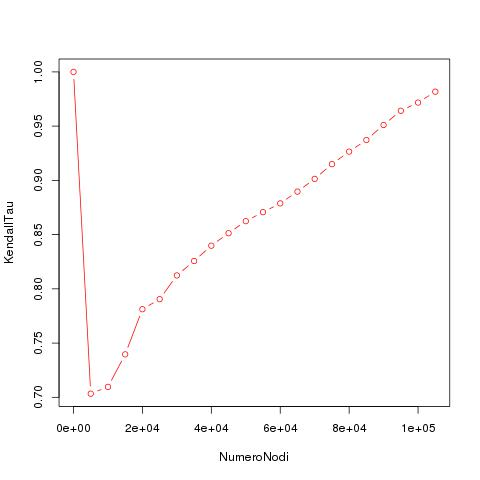
\includegraphics[height=9cm]{immagini/test1/trustranktestMode1_62}
 \caption{Test numero 1 (trustrank, 62). Calcolo della distanza dei vettori tra trustrank calcolato sull'intero grafo e trustrank calcolato sul grafo ricavato dai nodi visitati lungo una BFS partendo dal nodo 62.}
 \label{fig:test1trustModoB62}
\centering
 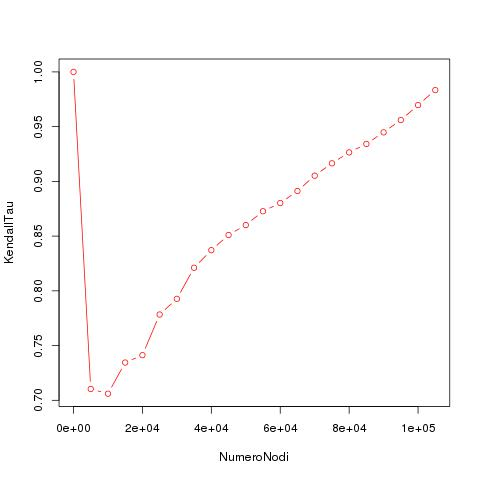
\includegraphics[height=9cm]{immagini/test1/trustranktestMode1_112}
 \caption{Test numero 1 (trustrank, 112). Calcolo della distanza dei vettori tra trustrank calcolato sull'intero grafo e trustrank calcolato sul grafo ricavato dai nodi visitati lungo una BFS partendo dal nodo 112.}
 \label{fig:test1trustModoB112}
\end{figure}

 \begin{figure}
\centering
 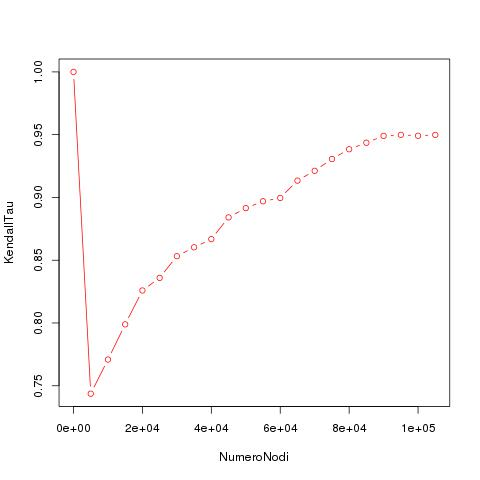
\includegraphics[height=9cm]{immagini/test1/antiTrustrankTestMode1_62}
 \caption{Test numero 1 (anti-trust rank, 62). Calcolo della distanza dei vettori tra anti-trust rank calcolato sull'intero grafo e anti-trust rank calcolato sul grafo ricavato dai nodi visitati lungo una BFS partendo dal nodo 62.}
 \label{fig:test1antitrustModoB62}
\centering
 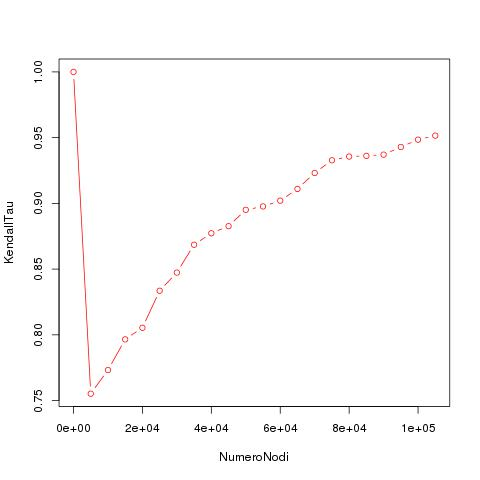
\includegraphics[height=9cm]{immagini/test1/antiTrustrankTestMode1_112}
 \caption{Test numero 1 (anti-trust rank, 112). Calcolo della distanza dei vettori tra anti-trust rank calcolato sull'intero grafo e anti-trust rank calcolato sul grafo ricavato dai nodi visitati lungo una BFS partendo dal nodo 112.}
 \label{fig:test1antitrustModoB112}
\end{figure}

Lo stesso test, applicato per valutare la distanza tra il vettore \(a\) di \textit{anti-trust rank} calcolato sull'intero grafo \(G\) e il vettore \(\hat{a}_i\) calcolato sul grafo temporaneo \(G_v\) ottenuto ad ogni intervallo di nodi visitati durante una visita in ampiezza \(v\), è illustrao in figura \ref{fig:test1antitrustModoB62} e in figura \ref{fig:test1antitrustModoB112}. Il primo grafico rappresenta la Tau di Kendall \(\tau_{a62}\)  dove il nodo sorgente della visita \(v\) è 62 mentre nel secondo grafico è illustrata la Tau di Kendall \(\tau_{a112}\) dove il nodo sorgente  della visita \(v\) è 112.  Sull'asse delle ascisse è rappresentato il numero di nodi che sono visitati durante la visita in ampiezza mentre sulle ordinate il corrispondente valore di Tau di Kendall \(\tau_a\). Anche in questo caso i due grafici hanno un andamento molto simile. Rispetto al test applicato a \textit{trustrank}, nel test di \textit{anti-trust rank}  i grafici (senza considerare il 
primo valore per lo stesso motivo dei due test precedenti) hanno un andamento quasi logaritmico dove il valore iniziale di Tau di Kendall 0.75 e  valore finali (stazionario) 0.95.

 \begin{figure}
\centering
 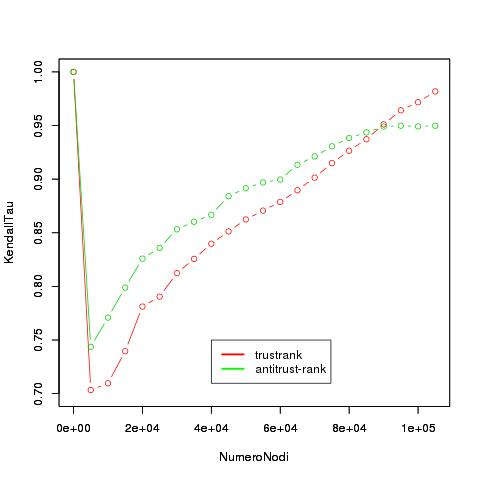
\includegraphics[height=9cm]{immagini/test1/coplotTrustAnti_62}
 \caption{Plotting del grafico \ref{fig:test1trustModoB62} e del  grafico \ref{fig:test1antitrustModoB62}}
 \label{fig:test1coplot62}
\centering
 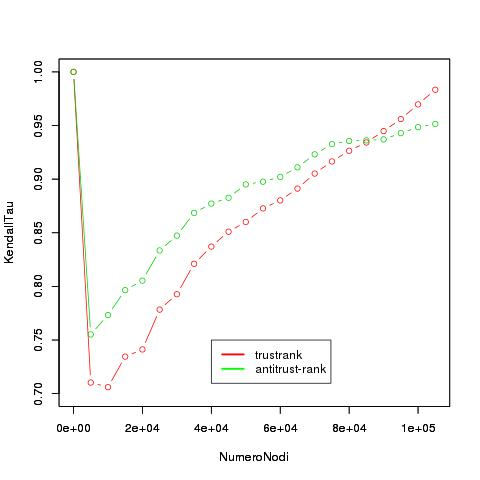
\includegraphics[height=9cm]{immagini/test1/coplotTrustAnti_112}
 \caption{Plotting del grafico \ref{fig:test1trustModoB112} e del  grafico \ref{fig:test1antitrustModoB112}}
 \label{fig:test1coplot112}
\end{figure}

In figura \ref{fig:test1coplot62} sono riportati in un unico grafico i grafici rappresentati in figura \ref{fig:test1trustModoB62}  e in figura \ref{fig:test1antitrustModoB62}; in rosso è rappresentato il grafico raffigurante la Tau di Kendall \(\tau_{t62}\) in verde è rappresentato il grafico  rappresentante la Tau di Kendall \(\tau_{a62}\). Si evince che inizialmente la Tau di Kendall \(\tau_{a62}\) tra il vettore \(a\) e il vettore \(\hat{a}_i\) cresce più velocemente rispetto alla Tau di Kendall \(\tau_{t62}\) applicata  tra il vettore \(t\) e il vettore \(\hat{t}_i\) ma dopo la visita di circa 80000 nodi la Tau di Kendall \(\tau_{t62}\) assume valori più alti rispetto a \(\tau_{a62}\) perché i valori di \(\tau_{a62}\) tendono a fermarsi a circa 0.95.\\
Il comportamento tra \(\tau_{t62}\) e \(\tau_{a62}\) indica perciò che \textit{trustrank} eseguito online è meno efficace di \textit{anti-trust rank} nell'approssimare il comportamento offline. Perciò tra questi due algoritmi quello che si adatta meglio nell'utilizzo in modalità online è \textit{anti-trust rank} perché tende ad approssimare fin da subito il comportamento offline anche avendo pochi nodi. Infatti il grafico in figura \ref{fig:test1coplot62} indica che \textit{anti-trust rank} eseguito durante la fase di crawling ritorna un vettore di valori che tendono ad avvicinarsi rapidamente ai valori del vettore di \textit{anti-trust rank} calcolato in modalità offline.\\
Le stesse valutazioni valgono tra il confronto dei due grafici in figura \ref{fig:test1trustModoB112} relativo a alla Tau di Kendall\(\tau_{t112}\) e \ref{fig:test1antitrustModoB112}  relativo alla Tau di Kendall \(\tau_{a112}\) illustrato in figura \ref{fig:test1coplot112}; in rosso è rappresentata la Tau di Kendall \(\tau_{t112}\) in verde è rappresentato il la Tau di Kendall \(\tau_{a112}\). Anche in questo caso \textit{anti-trust rank} online riesce ad approssimare bene  il comportamento offline già dall'inizio della visita in ampiezza (e quindi all'inizio del crawling), differentemente da \textit{trustrank} che non riesce ad avere le stesse prestazioni tranne quando la visita in ampiezza sul grafo \(G\) entra molto in profondità (nel caso esaminato dopo che sono stati visitati più di 80000 nodi su 114529). Quindi solo verso il termine della visita le prestazioni di \textit{trustrank} superano quelle di \textit{anti-trust rank}. Tali deduzioni si evincono dal fatto che \(\tau_{a112}\) cresce più 
rapidamente rispetto a \(\tau_{t112}\) ma solo dopo circa 80000 nodi \(\tau_{a112}\) cresce più lentamente rispetto a \(\tau_{
t112}\) che raggiunge valori più alti.



\section{Test 2}
Il test  calcola la distanza, utilizzando la Tau di Kendall \(\tau_t\), tra  il vettore \(t\) di \textit{trustrank} calcolato sull'intero grafo \(G\) e il vettore \(\hat{t}_i\) calcolato sul grafo temporaneo \(G_v\) ottenuto ad ogni intervallo di nodi visitati durante un visita in ampiezza \(v\). Quindi \(\tau_t\) viene calcolata ogni qual volta la visita in ampiezza \(v\) visita un certo intervallo di nodi da cui si ricava il grafo temporaneo \(G_v\) che è un sottografo di \(G\).  Anche per questo test l'intervallo è uguale a 5000.  Il test è molto simile al \textit{Test numero 1} ma differentemente del precedente nel calcolo della distanza tra i due vettori si esaminano i soli indici dei vettori \(t\) e \(\hat{t}_i\) che fanno riferimento ai nodi etichettati come spam. Ugualmente il test viene effettuato per valutare \textit{anti-trust rank} ma in questo caso vengono confrontati, tramite la Tau di Kendall \(\tau_a\), i soli nodi indici dei due vettori \(a\) e \(\hat{a}_i\) che fanno 
riferimento a nodi etichettati come non spam.\\
Dal momento che si devono confrontare i soli indici spam, nel calcolo di \(\tau_t\), i vettori \(t\) e \(\hat{t}_i\), durante il calcolo della distanza, sono ridimensionati ai soli indici etichettati spam. Lo stessa procedura è utilizzata  durante il calcolo di \(\tau_a\); in questo caso i vettori \(a\) e \(\hat{a}_i\) sono ridimensionati ai soli indici etichettati non spam. 

Il seedset usato per il calcolo di \textit{trustrank} è formato dall'insieme di nodi etichettati non spam del dataset WEBSPAM-UK2007 mentre il seedset usato per il calcolo di \textit{anti-trustrank} è composto dall'insieme dei nodi spam del dataset WEBSPAM-UK2007.

\begin{figure}
\centering
 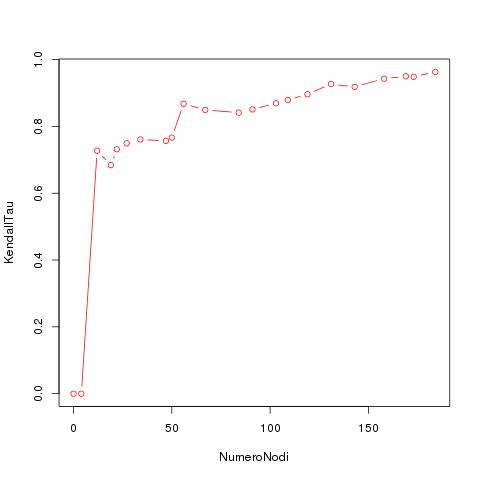
\includegraphics[height=9cm]{immagini/test2/trustrankBadNodesTestMode1_62}
 \caption{Test numero 2 (trustrank, 62). Calcolo della distanza dei vettori tra trustrank calcolato sull'intero grafo e trustrank calcolato sul grafo ricavato dai nodi visitati lungo una BFS partendo dal nodo 62 prendendo in considerazione i soli nodi spam. }
 \label{fig:test2trustModoB62}
\centering
 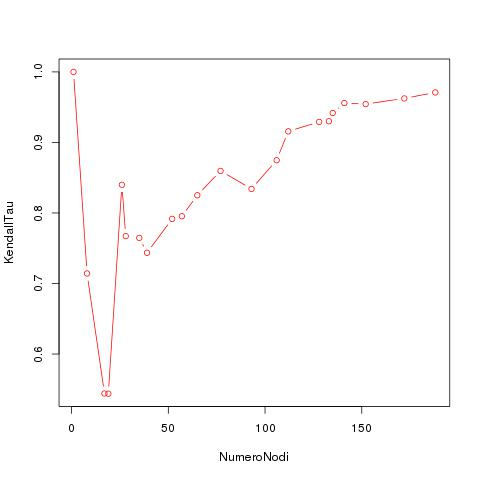
\includegraphics[height=9cm]{immagini/test2/trustrankBadNodesTestMode1_112}
 \caption{Test numero 2 (trustrank, 112). Calcolo della distanza dei vettori tra trustrank calcolato sull'intero grafo e trustrank calcolato sul grafo ricavato dai nodi visitati lungo una BFS partendo dal nodo 112 prendendo in considerazione i soli nodi spam.}
 \label{fig:test2trustModoB112}
\end{figure}

In figura \ref{fig:test2trustModoB62} è rappresentato il grafico del test rappresentante la Tua di Kendall \(\tau_{t62}\), calcolata tra gli indici spam dei vettori \(t\) e \(\hat{t}_i\), dove il nodo sorgente della visita in ampiezza, con cui viene ricavato il grafo temporaneo \(G_v\) è 62. Sull'asse delle ascisse è rappresentato il numero di nodi spam visitati durante la visita in ampiezza e sull'asse delle ordinate la Tau di Kendall \(\tau_{t62}\) calcolata a ogni intervallo di nodi visitati (compresi nodi spam e non spam).\\
Al primo passo, quando la visita in ampiezza ha visitato il solo nodo sorgente ci si aspetterebbe che il valore di \(\tau_{t62}\) sia  1 in quanto i vettori \(t\) e \(\hat{t}_i\) dovrebbero essere composti dal solo nodo visitato al primo passo (e quindi il nodo sorgente 62).  Ma dal momento che vengono presi in considerazione i soli nodi etichettati spam, il nodo 62 essendo etichettato non spam  viene scartato e quindi i vettori \(t\) e \(\hat{t}_i\) saranno vuoti e quindi si esplica perché \(\tau_{t62}\) al primo passo assume valore 0. Si noti che anche al secondo passo, quando il grafo temporaneo \(G_v\) è formato da 5001 nodi, la visita in ampiezza \(v\) non ha incontrato ancora nessun nodo spam e quindi \(\tau_{t62}\) è uguale a 0. Solo successivamente con l'avanzamento della visita in ampiezza  incontrando i nodi spam l'andamento del grafico cresce rapidamente fino a circa 0.7 per poi variare gradualmente fino a circa 1.0. 

\begin{figure}
\centering
 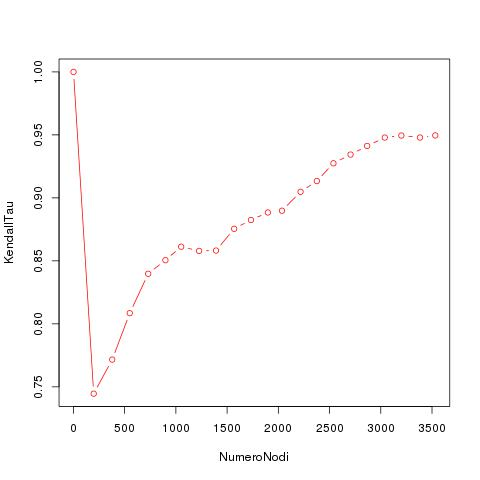
\includegraphics[height=9cm]{immagini/test2/antiTrustraktGoodNodesTestMode1_62}
 \caption{Test numero 2 (anti-trust rank, 62). Calcolo della distanza dei vettori tra anti-trust rank calcolato sull'intero grafo e anti-trust rank calcolato sul grafo ricavato dai nodi visitati lungo una BFS partendo dal nodo 62 prendendo in considerazione i soli nodi non spam. }
 \label{fig:test2antitrustModoB62}
\centering
 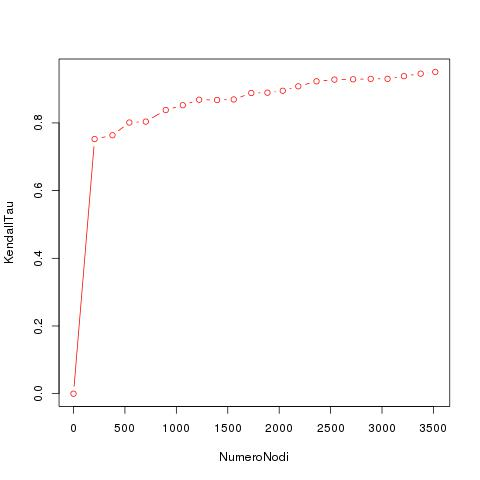
\includegraphics[height=9cm]{immagini/test2/antiTrustraktGoodNodesTestMode1_112}
 \caption{Test numero 2 (anti-trust rank, 112). Calcolo della distanza dei vettori tra anti-trust rank calcolato sull'intero grafo e anti-trust rank calcolato sul grafo ricavato dai nodi visitati lungo una BFS partendo dal nodo 112 prendendo in considerazione i soli nodi non spam. }
 \label{fig:test2antitrustModoB112}
\end{figure}

Il grafico della Tau di Kendall \(\tau_{t112}\)  calcolata  ad ogni intervallo di nodi visitati tramite la visita in ampiezza con nodo sorgente 112 è rappresentato in figura \ref{fig:test2trustModoB112}.  Sull'asse delle ascisse è rappresentato il numero dei soli nodi spam visitati tramite la visita in ampiezza e sull'asse delle ordinate la Tau di Kendall \(\tau_{t112}\) calcolata a ogni intervallo di nodi visitati (compresi nodi spam e non spam).\\
In questo caso il primo valore della Tau di Kendall \(\tau_{t112}\) è 1 perché, al primo passo della visita \(v\) si visita solo il nodo sorgente 112; quindi  i vettori \(t\) e \(\hat{t}_i\) saranno composti da un unico indice che fa riferimento al nodo 112 in quanto essendo spam tale nodo  viene considerato nella valutazione differentemente dal nodo 62; perciò, al primo passo di \(v\), \(\tau_{t112}\) è uguale a \ perché una Tau di Kendall applicata a vettori composti da un solo elemento produce come risultato 1. Successivamente con l'avanzamento della visita in ampiezza \(v\) l'andamento della Tau di Kendall \(\tau_{t112}\) calcolata su \(t\) e \(\hat{t}_i\) varia tra circa 0.5 e 1.

Lo stesso test è stato applicato per valutare \textit{anti-trust rank}; in figura \ref{fig:test2antitrustModoB62} è illustrato il grafico del test relativo alla Tau di Kendall \(\tau_{a62}\) per il calcolo della distanza tra il vettore \(a\) e il vettore \(\hat{a}_i\) prendendo in considerazione i soli nodi non spam e dove  la visita in ampiezza ha nodo sorgente 62. In figura \ref{fig:test2antitrustModoB112}, invece, è illustrato il grafico del test relativo alla Tau di Kendall \(\tau_{a112}\) che  calcola la distanza tra il vettore \(a\) e il vettore \(\hat{a}_i\) prendendo in considerazione i soli nodi non spam e dove la visita in ampiezza ha nodo sorgente 112. Sull'asse delle ascisse è rappresentato il numero dei soli nodi non spam incontrati tramite la visita in ampiezza tra tutti i nodi visitati e sull'asse delle ordinate la Tau di Kendall calcolato a ogni intervallo di nodi visitati.\\
Nel grafico in figura \ref{fig:test2antitrustModoB62} si nota che a differenza del test su \textit{trustrank} (rappresentato in figura \ref{fig:test1trustModoB62}), dove il nodo sorgente di \(v\) è 62, il primo valore della Tau di Kendall \(\tau_{a62}\), ovvero quando la visita in ampiezza ha visitato il solo nodo sorgente e quindi il grafo temporaneo \(G_v\) è formato dal solo nodo 62, è 1 perché in questo caso si esaminano i nodi non spam e tale nodo essendo non spam non viene rigettato ma viene esaminato; quindi i vettori \(a\) e\(\hat{a}_i\) avranno un solo indice relativo al nodo 62 e perciò la Tau di Kendall \(\tau_{a62}\) al primo passo sarà 1. Con l'aumentare dei nodi visitati i valori di \(\tau_{a62}\) varieranno da circa 0.75 a 0.95. \\
Il secondo grafico (figura \ref{fig:test2antitrustModoB112}) mentre ha come primo valore della Tau di Kendall \(\tau_{a112}\) uguale a 0, questo perché il grafo temporaneo \(G_v\) è formato, al primo passo,  dal solo nodo 112 e quindi dal momento che 112 è un nodo spam viene rigettato e non esaminato. Perciò in questo caso sia il vettore \(a\) che il vettore \(\hat{a}_i\) avranno lunghezza zero. Successivamente parallelamente all'avanzamento della visita in ampiezza il grafico varierà da circa 0.8 a circa 1.

%forse da eliminare
Dai test si deduce che  \textit{Anti-Trust Rank} è più efficace di \textit{Trustrank} in assoluto (vedi test 1) mentre \textit{Trustrank} è più efficace ad identificare i nodi spam; tale deduzione deriva  dal confronto dei grafici in figura \ref{fig:test2trustModoB62} e in figura \ref{fig:test2antitrustModoB62}. 

\section{Test 3}
Questo test è stato ideato in modo tale da simulare una situazione avversariale e mettere in difficoltà gli algoritmi di \textit{trustrank} e \textit{anti-trust rank} durante la loro esecuzione in modalità online. Si è pensato di simulare il caso in cui il seedset  utilizzato dagli algoritmi (il quale va a definire la distribuzione di probabilità rappresentata dal vettore di preferenza dell'algoritmo di \textit{trustrank} e \textit{anti-trust rank}) sia formato da nodi al limite del grafo \(G\).

Il test, quindi, consiste nell'eseguire una visita in ampiezza \(v_1\) da un nodo sorgente \(s\)  sull'intero grafo \(G\) e calcolare il vettore \(t_v\) di \textit{trustrank} sul grafo \(G_{v1}\), ricavato da tutti i nodi visitati alla fine della visita,  e dove il seedset \(S\) usato nel calcolo di \(t_v\) è composto dagli ultimi \(n\) nodi visitati da \(v_1\); dopodiché  si riesegue una seconda visita in ampiezza \(v_2\) con nodo sorgente \(s\) sul grafo \(G\) e si calcola il vettore \(\hat{t}_i\) di \textit{trustrank} sul grafo temporaneo \(G_{v2}\), ottenuto ad ogni intervallo di nodi visitati da \(v_2\), usando  come seedset \(S\) (ovvero l'insieme formato dagli ultimi \(n\) nodi visitati tramite la visita in ampiezza \(v_1\)).  Infine si calcola la Tau di Kendall \(\tau_t\) tra il vettore \(t_v\) e il vettore \(\hat{t}_i\) ad ogni intervallo di nodi che vengono visitati tramite la visita in ampiezza \(v_2\).\\
Lo stesso test è stato applicato per valutare \textit{anti-trust rank}. In questo caso si esegue una visita in ampiezza \(v_1\) da un nodo sorgente \(s\) sull'intero grafo \(G\) e viene calcolato il vettore \(a_v\) di \textit{anti-trust rank} sul grafo \(G_{v1}\), composto da tutti i nodi visitati alla fine della visita, e  il seedset \(S\) utilizzato per il calcolo di \(a_v\) sarà composto dagli ultimi \(n\) nodi visitati da \(v_1\); successivamente si riesegue una seconda visita in ampiezza \(v_2\) con nodo sorgente \(s\) e si calcola il vettore \(\hat{a}_i\) di \textit{anti-trust rank} sul grafo temporaneo \(G_{v2}\) ottenuto ad ogni intervallo di nodi visitato tramite la \(v_2\). Anche in questo caso il seedset per calcolare \(\hat{a}_i\) è formato dell'insieme \(S\). Infine  viene calcolata la Tau di Kendall \(\tau_a\) tra il vettore \(a_v\) e il vettore \(\hat{a}_i\) per ogni intervallo di nodi che vengono visitati tramite la visita in ampiezza \(v_2\).\\
Durante il calcolo di \(\hat{t}_i\) e di \(\hat{a}_i\), sul grafo temporaneo \(G_{v2}\) ottenuto dai nodi lungo la visita in ampiezza \(v_2\), se ad un certo passo \(p\) la visita \(v_2\) non  è arrivata ai nodi dell'insieme \(S\) all'estremo del grafo \(G\), allora il vettore di preferenza con cui si calcolerà \(\hat{t}_i\) e \(\hat{a}_i\) sarà una distribuzione uniforme. Se il vettore di preferenza è costituito da una distribuzione uniforme allora il calcolo di \textit{trustrank} è equivalente a \textit{pagerank} mentre il calcolo di \textit{anti-trustrank} è equivalente \textit{pagerank} trasposto. Nel momento in cui la visita in ampiezza incomincerà ad incontrare qualche nodo dell'insieme \(S\) allora il vettore di preferenza verrà manipolato con una distribuzione personalizzata basata sui nodi appartenenti all'insieme \(S\) visitati. \\
Il numero di  nodi utilizzato per definire l'insieme \(S\) è 3776 come la grandezza dell'insieme delle pagine etichettate non spam nel dataset WEBSPAM-UK2007. E l'intervallo scelto da cui si ricava il grafo temporaneo \(G_{v_2}\) è 500; quindi ogni 500 nodi visitati dalla visita in ampiezza \(v_2\) viene definito un nuovo grafo temporaneo \(G_{v_2}\) sottografo di \(G\) su cui viene calcolato \(\hat{t}_i\) e \(\hat{a}_i\).
\begin{figure}
\centering
 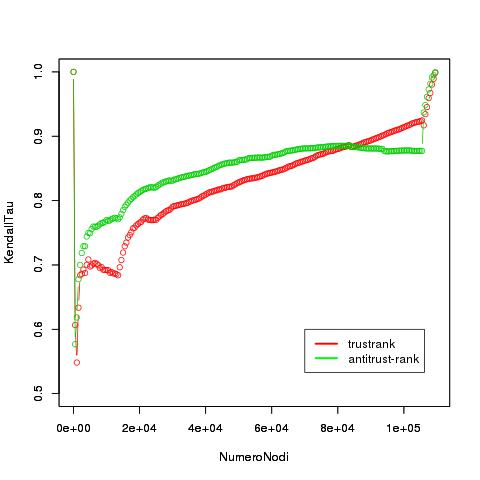
\includegraphics[height=9cm]{immagini/test3/coplotTrustAnti_Mode1_set3776_62}
 \caption{Test numero 3 . In rosso, calcolo della Tau di Kendall  tra il vettore $t_v$ e il vettore $\hat{t}_i$ per ogni intervallo di nodi visitati della BFS partendo dal nodo 62. In verde calcolo della Tau di Kendall tra il vettore $a_v$ e il vettore $\hat{a}_i$ per ogni intervallo di nodi visitati della BFS partendo dal nodo 62}
 \label{fig:test3coplotTrustAntiModeB62}
\end{figure}

In figura \ref{fig:test3coplotTrustAntiModeB62} è rappresentato il grafico del test eseguito per valutare \textit{trustrank} e \textit{anti-trust rank}; in particolare nel grafico è illustrata, in verde, la Tau di Kendall \(\tau_{t62}\) tra il vettore \(t_v\) e il vettore \(\hat{t}_i\) , e in rosso la Tau di Kendall \(\tau_{a62}\) tra il vettore \(a_v\) e il vettore \(\hat{a}_i\); in entrambi i test il nodo sorgente delle visite in ampiezza \(v_1\) e \(v_2\), da cui si ricavano i grafi \(G_{v1}\) e \(G_{v_2}\), è 62. Sull'asse delle ascisse è rappresentato il numero di nodi visitati tramite la visita \(v_2\) mentre sull'asse delle ordinate il valore delle Tau di Kendall \(T_{t62}\) e \(T_{a62}\).\\
Il primo valore delle Tau di Kendall \(\tau_{t62}\) e \(\tau_{a112}\) è 1 per il fatto che la vista \(v_2\) al primo passo  incontra il solo nodo sorgente perciò al passo uno il grafo temporaneo sarà composto dal solo nodo 62 e i vettori \(t_v\) e \(\hat{t}_i\), nel calcolo di \(\tau_{t62}\), e i vettori \(a_v\) e \(\hat{a}_i\), nel calcolo di \(\tau_{a62}\), saranno composti da un solo indice relativo al nodo sorgente 62 e quindi le Tau di Kendall ritorneranno valore 1.

Dopo aver visitato il primo nodo, tramite la visita in ampiezza \(v_2\), i valori della Tau di Kendall \(\tau_{t62}\) crescono da circa 0.55  e salgono gradualmente fino ad arrivare a 0.9 quando \(v_2\) visitata 105790 nodi. Dopo che  la visita \(v_2\) incontra 105790 nodi i valori della Tau di Kendall \(\tau_{t62}\) crescono rapidamente fino a toccare 1 al termine della visita (ovvero dopo 109566 nodi). Questo comportamento si spiega dal fatto che la visita in ampiezza con nodo dorgente 62 incontra un totale di 109566 nodi (su 114529 totali del grafo \(G\)) e dal momento che il seedset \(S\) è formato dagli ultimi 3776 nodi incontrati dalla visita allora fino a 109570 il vettore di preferenza con cui è calcolato \(\hat{t}_i\) è uguale a una distribuzione uniforme mentre dopo aver visitato 109570 nodi il vettore di preferenza cambia e verrà manipolato tramite i nodi incontrati facenti parte dell'insieme \(S\). Quindi dopo aver visitato 109570 nodi i valori della Tau di Kendall \(\tau_{t62}\) salgono 
rapidamente perché il seedset con cui è stato calcolato \(t_v\) e il seedset con cui viene calcolato \(\hat{t}_i\) tendono a essere sempre più simili tanto più la visita \(v_2\) incontra i nodi all'interno dell'insieme \(S\) ed inoltre anche i grafi su cui vengono calcolati \(t_v\) e \(\hat{t}_i\) tendono ad essere identici. Lo stesso comportamento è riscontrabile per la Tau di Kendall \(\tau_{a62}\) (per l'analisi di \textit{anti-trust rank}).\\ 
Anche se i comportamenti delle delle Tau di Kendall \(\tau_{t62}\) e \(\tau_{a62}\) sono molto simili, la loro crescita è differente; la Tau di Kendall \(\tau_{a62}\) cresce più rapidamente rispetto alla Tau di Kendall \(\tau_{t62}\) la quale cresce più lentamente ma tale comportamento cambia dopo che \(v_2\) ha incontrato circa 80000 nodi.\\
Quindi si evince che \textit{anti-trust rank} è meno dipendente dal vettore di preferenza che gli viene passato rispetto a \textit{trustrank}, almeno fino a quando il grafo temporaneo è al massimo l'80\% del grafo completo. Quindi anche se si usasse \textit{anti-trust rank} in modalità online con un seedset poco pertinente questo riuscirebbe a produrre, fin dall'inizio del crawling, dei risultati molto vicini a quelli calcolati da \textit{anti-trust rank} sull'intero grafo con un altro seedset. Mentre \textit{trustrank} non riesce ad approssimare bene tale comportamento rispetto ad \textit{anti-trust rank} tranne quando il  grafo temporaneo incomincia a diventare sufficientemente grande.

\section{Test 4}
Questo test ha la stessa struttura del \textit{test numero 3} dove, però,  il vettore \(t_v\) di \textit{trustrank}, calcolato sul grafo \(G_{v1}\) ricavato dai nodi al termine della visita in ampiezza \(v_1\) con nodo sorgente \(s\)  sul grafo \(G\), e il vettore \(\hat{t_i}\), calcolato sul grafo temporaneo \(G_{v2}\) ricavato ad ogni intervallo di nodi visitati tramite la visita \(v_2\) con nodo sorgente \(s\), sono ottenuti usando il fattore di attenuazione \(\alpha\) impostato a 0.005. Lo stesso test è stato applicato per analizzare \textit{anti-trust rank}. Come per il test precedente il nodo sorgente delle visite in ampiezza \(v_1\) e \(v_2\) è 62  e il seedset con cui sono eseguiti \textit{trustrank} e \textit{anti-trust rank} è composto dagli ultimi \(n\) nodi (dove \(n\) è uguale a 3776)  incontrati tramite la visita in ampiezza \(v_1\).\\
Il fattore \(\alpha\) impostato ad un valore molto vicino allo 0 aumenta la probabilità che \textit{trustrank} o \textit{anti-trust rank}  privilegino la distribuzione descritta dal vettore di preferenza invece di seguire un semplice cammino sul grafo (per maggiori chiarimenti si consiglia di leggere il paragrafo \ref{sub:esogeno} dove è descritto \textit{Pagerank}).


In figura \ref{fig:test4coplotTrustAntiModeB620005} è illustrato il grafico della Tau di Kendall \(\tau_{t62}\) tra \(t_v\) e \(\hat{t}_i\) (in rosso)  e della Tau di Kendall \(\tau_{a62}\) tra \(a_v\) e \(\hat{a}_i\) (in verde). Sull'asse delle ascisse è rappresentato il numero di nodi visitati tramite la visita \(v_2\) mentre sull'asse delle ordinate il valore delle Tau di Kendall \(\tau_{t62}\) e \(\tau_{a62}\). Come si nota dal grafico dopo il primo passo della visita \(v_2\), dove \(\tau_{t62}\) assume valore 1, \(\tau_{t62}\) varia da circa 0.5 (all'inizio della visita) a circa 0.75 (quando la visita incontrato 109570 nodi);  dopo che la visita \(v_2\) incontra i primi nodi  \(S\) (dopo 109570) allora \(\hat{t}_i\) tende ad avere valori sempre più simili a \(t_v\) fino ad arrivare a 1 quando tutti i nodi in \(S\) sono stati visitati tramite \(v_2\) e quindi  \(\hat{t_i}\) sarà calcolato con un seedset uguale all'intero inseme \(S\). La crescita vertiginosa di \(\tau_{t62}\), dopo che \(v_2\) supera 
109570 nodi, dipende sia dal fatto che la visita \(v_2\) è entrata molto in profondità, e quindi il grafo temporaneo \(G_{v2}\) su cui viene calcolato \(\hat{t}_i\) è molto simile al grafo \(G_v\), e sia dal fatto che i seedset con cui sono calcolati \(t\) e \(\hat{t}_i\) tendono ad essere sempre più simili con l'avanzare della visita.\\ 
Questo comportamento non si evince per la Tau di Kendall \(\tau_{a62}\) la quale assume valori più bassi  e tende a non crescere fino al momento in cui la visita \(v_2\) non incontra i primi nodi del seedset \(S\) (dopo 109570 nodi). Il grafico indica che quanto più la visita in ampiezza \(v_2\) entra in profondità i due vettori \(a_v\) e \(\hat{a}_i\) sono sempre più distanti e solo dopo che \(v_2\) incomincia ad incontrare i nodi \(S\) e il seedset con cui \(\hat{a}_i\) viene calcolato è rimpiazzato dai nodi visitati in \(S\), la Tau di Kendall \(\tau_{a62}\) incomincia a crescere fino ad arrivare a 1 quando tutti i nodi  in \(S\) sono stati visitati.
\begin{figure}
 \centering
 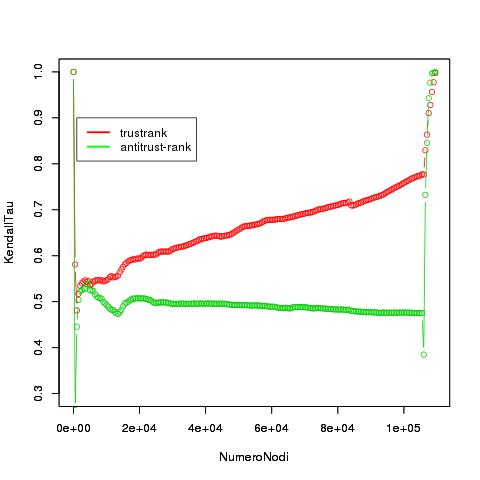
\includegraphics[height=9cm]{immagini/test4/coplotTrustAnti_Mode1_set3776_62_alpha0005}
  \caption{Test numero 4 . In rosso, calcolo della Tau di Kendall tra il vettore $t_v$ e il vettore $\hat{t}_i$, dove $\alpha$ è impostato a 0.005. In verde calcolo della Tau di Kendall tra il vettore $a_v$ e il vettore $\hat{a}_i$, dove $\alpha$ è impostato a 0.005.}
 \label{fig:test4coplotTrustAntiModeB620005}
\end{figure}

%inserire ragionamento perché si ottengono i risultati nel test3 e test4, forse è dovuto al fatto che antitrustrank è calcolato sul grafo trasposto

\section{Test 5}
Il seguente test, ad ogni intervallo di nodi visitati tramite una visita in ampiezza \(v\)  con nodo sorgente \(s\) sul grafo \(G\), calcola il vettore \(\hat{t}_i\) di \textit{trustrank}  sul grafo temporaneo \(G_v\), ottenuto dai nodi visitato da \(v\), e successivamente calcola la differenza \(\Delta_t\) tra la media \(Mb_t\) dei valori di \(\hat{t}_i\) dei nodi etichettati non spam, e la media \(Ms_t\) dei valori di \(\hat{t}_i\) dei nodi etichettati spam . Quindi per ogni intervallo di nodi visitato tramite la visita in ampiezza \(v\) si calcola:
\begin{equation}
 \Delta_t = Mb_t-Ms_t
\end{equation}

Lo stesso test è applicato per analizzare \textit{anti-trust rank}; ad ogni intervallo di nodi visitato  tramite la visita in ampiezza \(v\) con nodo sorgente \(s\) sul grafo \(G\), viene calcolato il vettore \(\hat{a}_i\)  di \textit{anti-trust rank}  sul grafo temporaneo \(G_v\), ottenuto dai nodi della visita \(v\);  dopodiché viene calcolata la differenza \(\Delta_a\) tra la media \(Mb_a\) dei valori di \(\hat{a}_i\) dei nodi non spam, e la media \(Ms_a\) dei valori di \(\hat{a}_i\) dei nodi etichettati spam. Perciò \(\Delta_a\) sarà uguale a:
\begin{equation}
 \Delta_a=Mb_a-Ms_a
\end{equation}

 
\begin{figure}
 \centering
 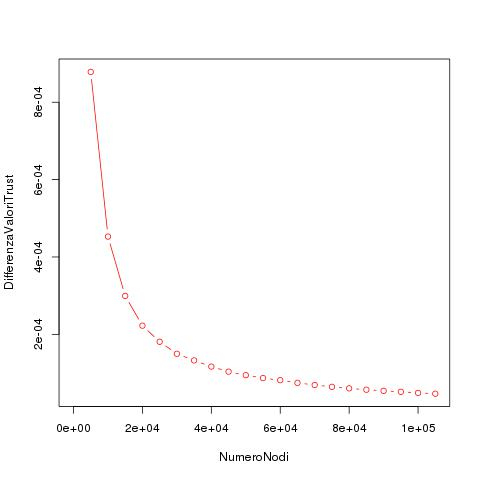
\includegraphics[height=9cm]{immagini/test5/averageTest_trust_62}
  \caption{Test 5 (trustrank,62). Differenza tra le medie dei valori di trustrank, calcolati sul grafo temporaneo ottenuto ad ogni intervallo di nodi visitati tramite la visita in ampiezza con nodo sorgente 62, dei nodi non spam e nodi spam.}
 \label{fig:test5trust62}
  \centering
 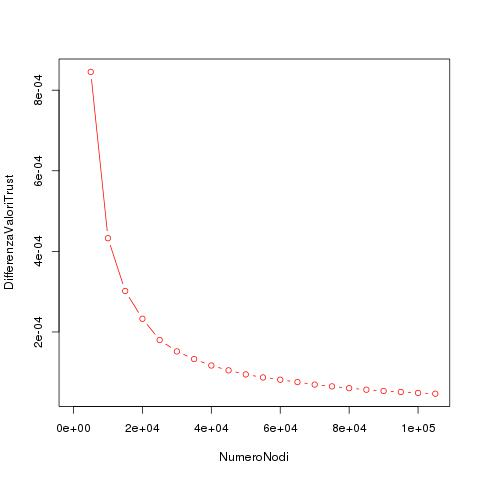
\includegraphics[height=9cm]{immagini/test5/averageTest_trust_112}
  \caption{Test 5 (trustrank,112). Differenza tra le medie dei valori di trustrank, calcolati sul grafo temporaneo ottenuto ad ogni intervallo di nodi visitati tramite la visita in ampiezza con nodo sorgente 112, dei nodi non spam e nodi spam.}
 \label{fig:test5trust112}
\end{figure}

Un algoritmo di spam detection come \textit{trustrank} e \textit{anti-trust rank} dovrebbe identificare bene il gruppo di nodi spam dal gruppo dei nodi spam assegnando valori molto distanti tra i due gruppi. Quindi ci si dovrebbe aspettare che i nodi etichettati spam dai nodi etichettati non spam abbiano dei valori differenti e distanti tra loro; quindi nel caso di \textit{trustrank} i nodi etichettati non spam dovrebbero avere valori più alti rispetto ai nodi etichettati spam, mentre nel caso di  \textit{anti-trust rank} dovrebbe succedere il contrario.\\
Perciò, nel caso di \textit{trustrank} ci si aspetta, che  il calcolo di \(\hat{t}_i\) sul grafo temporaneo \(G_v\) ottenuto ai primi passi della visita \(v\) dovrebbe restituire dei valori di \textit{trustrank} per i nodi non spam e per i nodi spam abbastanza vicini in quanto il grafo \(G_v\) è troppo piccolo per poter calcolare dei valori \(\hat{t}_i\) molto affidabili. Quindi la differenza \(\Delta_t\) ai primi passi della visita dovrebbe essere molto piccola. Il valore della differenza \(\Delta_t\) dovrebbe crescere proporzionalmente alla visita e quindi alla fine della visita, quando il grafo temporaneo \(G_v\) è composto dalla maggior parte dei nodi dell'intero grafo \(G\), la distanza tra i valori di \textit{trustrank} dei nodi non spam dai valori di \textit{trustrank} dei nodi spam dovrebbero essere maggiore. Quindi i nodi non spam dovrebbero avere valori più alti di \textit{trustrank} (dal momento che \textit{trustrank} determina il livello di affidabilità di un nodo) rispetto ai nodi spam. Perciò 
la 
differenza tra la media \(Mb_t\) dei valori di \textit{trustrank} dei nodi non spam con la media \(Ms_t\) dei valori di \textit{trustrank} dei nodi spam dovrebbe essere più grande rispetto all'inizio della visita. Si deduce quindi che durante la visita \(v\), \(Mb_t\) dovrebbe crescere e \(Ms_t\) dovrebbe decrescere.\\
Nel caso di \textit{anti-trust rank} ci si aspetta  che \(\hat{a}_i\) calcolato all'inzio della visita \(v\) restituisca dei valori per i nodi non spam e per i nodi spam molto vicini e quindi \(\Delta_a\) dovrebbe  essere prossima allo zero. Ma differentemente da quanto accade per \textit{trustrank}, \(\hat{a}_i\) calcolato verso la fine della visita \(v\) dovrebbe restituire dei valori per i nodi non spam molto piccoli (perché \textit{anti-trust rank} indica la probabilità  che un nodo sia spam) e per i nodi spam dei valori molto alti. Si deduce quindi che alla fine della visita \(v\),  \(Mb_a\) dovrebbe essere più piccola di \(Ms_a\) e di conseguenza che \(\Delta_a\) dovrebbe essere negativa . 

In figura \ref{fig:test5trust62} e in figura \ref{fig:test5trust112} è illustrato il test rappresentate la differenza \(\Delta_t\); nel primo grafico \(\Delta_t\) è calcolata attraverso una visita in ampiezza con nodo sorgete 62 mentre nel secondo grafico \(\Delta_t\) è calcolata tramite una visita in ampiezza con nodo sorgente 112. I risultati dei grafici smentiscono il comportamento di \textit{trustrank} descritto in precedenza in quanto all'inizio della visita la differenza \(\Delta_t\), tra la media dei valori di  \(\hat{t}_i\) dei nodi non spam e la media dei valori di \(\hat{t}_i\)  dei  nodi spam , ha un valore più alto rispetto alla differenza \(\Delta_t\) calcolata sul grafo temporaneo che si ottiene ai passi successivi della visita in ampiezza. Tale comportamento implica che la distanza tra i valori di \textit{trustrank} tra i nodi non spam e spam tende ad essere meno marcata quando \textit{trustrank} viene calcolato sul grafo temporaneo composto da quasi tutti i nodi dell'intero grafo (infatti la 
curva 
tende a 
decrescere). Perciò invece di avere un andamento logaritmo i grafici sono contraddistinti da una parabola decrescente.

\begin{figure}
 \centering
 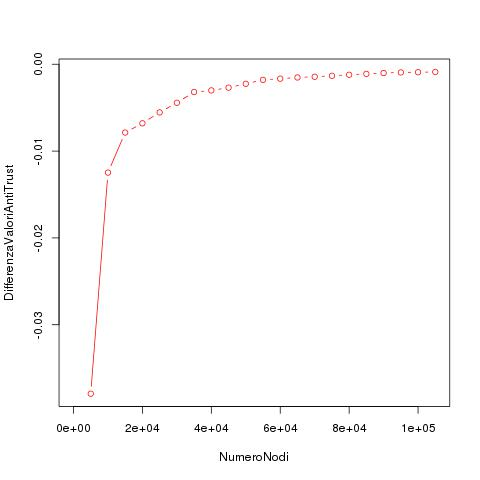
\includegraphics[height=9cm]{immagini/test5/averageTest_antitrust_62}
  \caption{Test 5 (anti-trust rank,62). Differenza tra le medie dei valori di anti-trust rank, calcolati sul grafo temporaneo ottenuto ad ogni intervallo di nodi visitati tramite la visita in ampiezza con nodo sorgente 62, dei nodi non spam e nodi spam.}
 \label{fig:test5antitrust62}
  \centering
 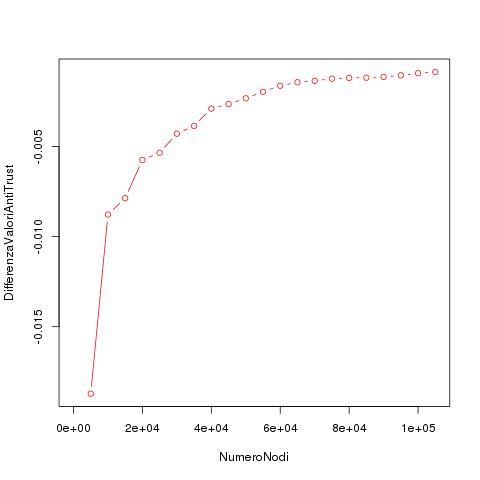
\includegraphics[height=9cm]{immagini/test5/averageTest_antitrust_112}
  \caption{Test 5 (anti-trust rank,112). Differenza tra le medie dei valori di anti-trust rank, calcolati sul grafo temporaneo ottenuto ad ogni intervallo di nodi visitati tramite la visita in ampiezza con nodo sorgente 112, dei nodi non spam e nodi spam.}
 \label{fig:test5antitrust112}
\end{figure}

In figura \ref{fig:test5antitrust62} e in figura \ref{fig:test5antitrust112} sono illustrati i grafici del test rappresentate la differenza \(\Delta_a\). Nel primo grafico il nodo sorgente della visita in ampiezza \(v\) è 62 nel secondo è 112. Anche in questo caso i risultati illustrati nei due grafici smentiscono il comportamento atteso in quanto il valore di \(\Delta_a\) aumenta con l'aumentare dei nodi del grafo temporaneo su cui viene calcolato \(\hat{a}_i\). Tale risultato indica che il calcolo di \(\hat{a}_i\) sul grafo temporaneo ottenuto ai primi passi della visita (e quindi con pochi nodi) discrimina più fortemente i nodi non spam da 
quelli spam. Infatti la differenza \(\Delta_a\) cresce da circa -0.004 a circa 0 con l'avanzare della visita; perciò con l'aumentare dei nodi del grafo temporaneo \(G_v\), su cui viene calcolato \(\hat{a}_i\), la media dei valori \(\hat{a}_i\) dei nodi non spam tende a crescere fino ad essere molto simile alla media dei valori \(\hat{a}_i\) dei nodi spam che tende a decrescere.

%chiedere da eliminare
Dal test si deduce che \textit{TrustRank} è più efficace nella ricerca dei nodi spam (e quindi vengono confermati i risultati del test 2) perhé con l'avanzare della visita la media dei nodi spam tende a crescere. Inoltre si evince che \textit{Anti-Trust Rank} è più efficace nell'identificare i nodi non spam in quanto con l'avanzare della visita la media dei nodi non spam cresce fino a diventare molto vicina alla media dei nodi spam.


\section{Test 6}
Dal momento che il \textit{test numero 5} ha prodotto dei risultati che indicano un comportamento diverso da quello atteso, è stato implementato questo test per verificare la correttezza dei risultati ottenuti. Il test consiste nell'esecuzione di una visita in ampiezza \(v\) sul grafo \(G\) del dataset preso in esame con nodo sorgente \(s\) (dove il nodo sorgente è 62 e  112) e per ogni intervallo di nodi visitati si ricava il grafo temporaneo \(G_v\). Quindi si determinano i nodi etichettati non spam e spam del grafo temporaneo e utilizzando il loro valore di \textit{trustrank} finale nel vettore \(t\), calcolato sull'intero grafo \(G\), si calcola la differenza \(\Delta_t\)   tra la media \(Mb_t\), dei valori dei nodi non spam, e la media \(Ms_t\), dei valori dei nodi spam,  del grafo \(G_v\).\\
Il test è applicato anche per valutare \textit{anti-trust rank}; in questo caso ad ogni passo della visita in ampiezza \(v\) sul grafo \(G\) con nodo sorgente \(s\) (anche in questo caso il nodo sorgente è 62 e  112) e per ogni intervallo di nodi visitati tramite la visita \(v\) si ricava il grafo temporaneo \(G_v\); quindi si determinano i nodi etichettati non spam e spam del grafo temporaneo e utilizzando il loro valore di \textit{anti-trust rank} finale nel vettore \(a\), calcolato sull'intero grafo \(G\), si calcola la differenza \(\Delta_a\)   tra la media \(Mb_a\), dei valori dei nodi non spam, e la media \(Ms_a\), dei valori dei nodi spam,  del grafo \(G_v\).
\begin{figure}
 \centering
 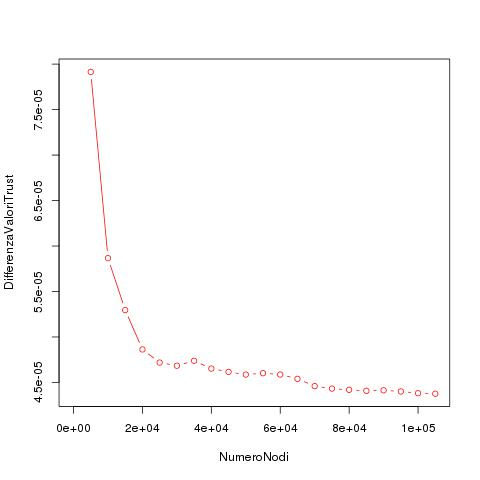
\includegraphics[height=9cm]{immagini/test6/averageCompleteTest_trust_62}
  \caption{Test 6 (trustrank,62). Differenza tra la media dei valori di trustrank finali dei nodi non spam e la media dei valori di trustrank nodi spam, per ogni intervallo di nodi visitati tramite la visita in ampiezza con nodo sorgente 62.}
 \label{fig:test6trust62}
  \centering
 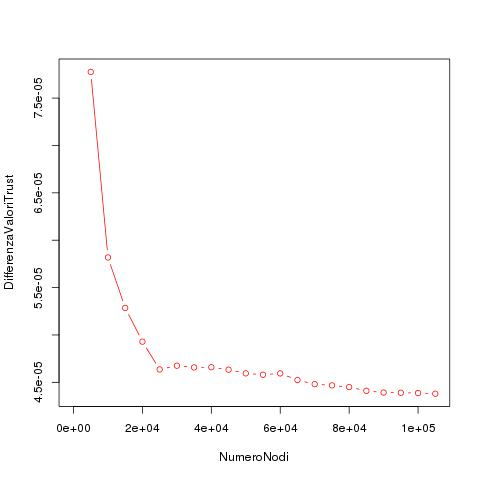
\includegraphics[height=9cm]{immagini/test6/averageCompleteTest_trust_112}
  \caption{Test 6 (trustrank,112). Differenza tra la media dei valori di trustrank finali dei nodi non spam e la media dei valori di trustrank nodi spam, per ogni intervallo di nodi visitati tramite la visita in ampiezza con nodo sorgente 112.}
 \label{fig:test6trust112}
\end{figure} 
\begin{figure}
 \centering
 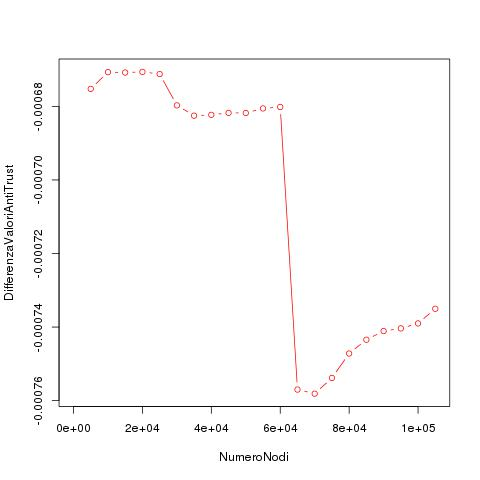
\includegraphics[height=9cm]{immagini/test6/averageCompleteTest_antitrust_62}
  \caption{Test 6 (anti-trust rank,62). Differenza tra la media dei valori di trustrank finali dei nodi non spam e la media dei valori di trustrank nodi spam, per ogni intervallo di nodi visitati tramite la visita in ampiezza con nodo sorgente 62.}
 \label{fig:test6antitrust62}
  \centering
 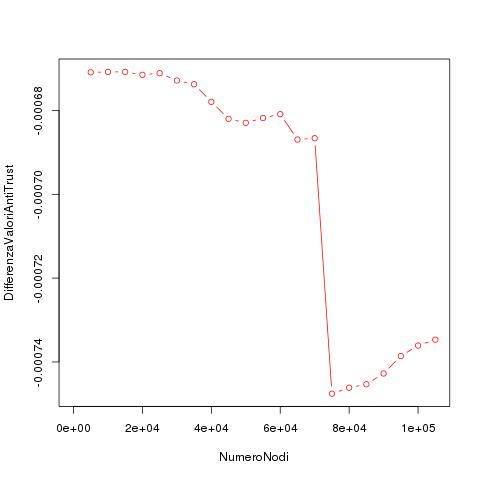
\includegraphics[height=9cm]{immagini/test6/averageCompleteTest_antitrust_112}
  \caption{Test 6 (anti-trust rank,112). Differenza tra la media dei valori di trustrank finali dei nodi non spam e la media dei valori di trustrank nodi spam, per ogni intervallo di nodi visitati tramite la visita in ampiezza con nodo sorgente 112.}
 \label{fig:test6antitrust112}
\end{figure}

Quindi si vuole verificare se i risultati ottenuti dall'analisi tramite il \textit{test numero 5}, sono dipendenti dai valori calcolati sull'intero grafo \(G\) di \textit{trustrank}.

In figura \ref{fig:test6trust62} è illustrato il grafico del test rappresentante \(\Delta_t\) dove il nodo sorgente della visita in ampiezza \(v\) è 62 mentre in figura \ref{fig:test6trust112} è illustrato il grafico del test rappresentante \(\Delta_t\) dove il nodo sorgente della visita in ampiezza è 112. In entrambi i grafici sull'asse delle ascisse è rappresentato il numero di nodi visitati tramite la visita in ampiezza mentre sull'asse delle ordinate è rappresentata \(\Delta_t\) calcolata ad ogni intervallo di nodi visitato attraverso la visita in ampiezza. L'andamento dei grafici giustifica i risultati ottenuti nel \textit{test numero 5} illustrati in figura \ref{fig:test5trust62} e in figura \ref{fig:test5trust112}, i quali hanno un andamento molto simile. Un fattore importante che evince nel confronto con i grafici precedenti è il range in cui variano i valori \(\Delta_t\); in questo test il range è di un ordine di grandezza più piccolo e quindi si deduce che la media dei valori di \textit{trustrank} 
del gruppo di nodi spam e la media di \textit{trustrank} del gruppo di nodi non spam, contrariamente a quanto ci si aspetta, sono molto vicine. Perciò il test conferma il fatto che \textit{trustrank} calcolato sull'intero grafo \(G\) non discrimina fortemente i nodi spam da quelli non spam e che quindi i risultati ottenuti nel \textit{test numero 5} dipendono dall'algoritmo di \textit{trustrank}.

Oltre alla valutazione di \textit{trustrank}, in figura \ref{fig:test6antitrust62}  è illustrato il grafico del test rappresentante \(\Delta_a\) dove il nodo sorgente della visita in ampiezza è 62 e in figura \ref{fig:test6antitrust112} è illustrato il grafico del test rappresentante \(\Delta_a\) dove il nodo sorgente della visita in ampiezza è 112. In entrambi i grafici sull'asse delle ascisse è rappresentato il numero di nodi visitati tramite la visita in ampiezza mentre sull'asse delle ordinate è rappresentata \(\Delta_a\) calcolata ad ogni intervallo di nodi visitato attraverso la visita in ampiezza. Dai grafici si evince che  \(\Delta_a\)  ha un comportamento al quanto ambiguo; ovvero nel grafico in figura \ref{fig:test6antitrust62}, vi è un salto di circa 0.00008 unità, dopo circa 60000 nodi visitati attraverso la visita in ampiezza \(v\), mentre nel secondo vi è un salto di circa 0.00006 unità, dopo circa 780000 nodi visitati \(v\). Ma dal momento che i  valori dei grafici in figura \ref{fig:test6antitrust62} e in figura \ref{fig:test6antitrust112}, variano in un range molto piccolo possono confermare i risultati ottenuti nel \textit{test numero 5}  ovvero alla fine della visita la distanza tra la media dei valori di \textit{anti-trust rank} del gruppo di nodi spam e la media di \textit{anti-trust rank} del gruppo di nodi spam è meno marcata.

